\documentclass[tikz,border=8pt]{standalone}
% Shared look for every TikZ diagram. Load with \input{../../tools/tikz-style.tex}
\usepackage[T1]{fontenc}
\usepackage{lmodern}
\renewcommand{\sfdefault}{lmr}  % diagrams use the same serif as the text
\usetikzlibrary{arrows.meta, positioning, shapes.geometric, calc, fit, backgrounds}
\definecolor{cblue}{HTML}{4C78A8}
\definecolor{corange}{HTML}{F58518}
\definecolor{cgreen}{HTML}{54A24B}
\definecolor{cred}{HTML}{E45756}
\definecolor{cpurple}{HTML}{B279A2}
\definecolor{cgrey}{HTML}{6B6B6B}
\tikzset{
  every picture/.style={font=\sffamily, line width=1.2pt},
  box/.style={draw=#1, fill=#1!12, rounded corners=4pt, align=center, inner sep=7pt, minimum height=1.1cm},
  box/.default=cgrey,
  arrow/.style={-{Stealth[length=3mm]}, draw=cgrey, line width=1.4pt},
  title/.style={font=\sffamily\bfseries\Large},
  note/.style={font=\sffamily\small, text=cgrey, align=center},
}
\AtBeginDocument{\hyphenpenalty=10000 \exhyphenpenalty=10000}

\begin{document}
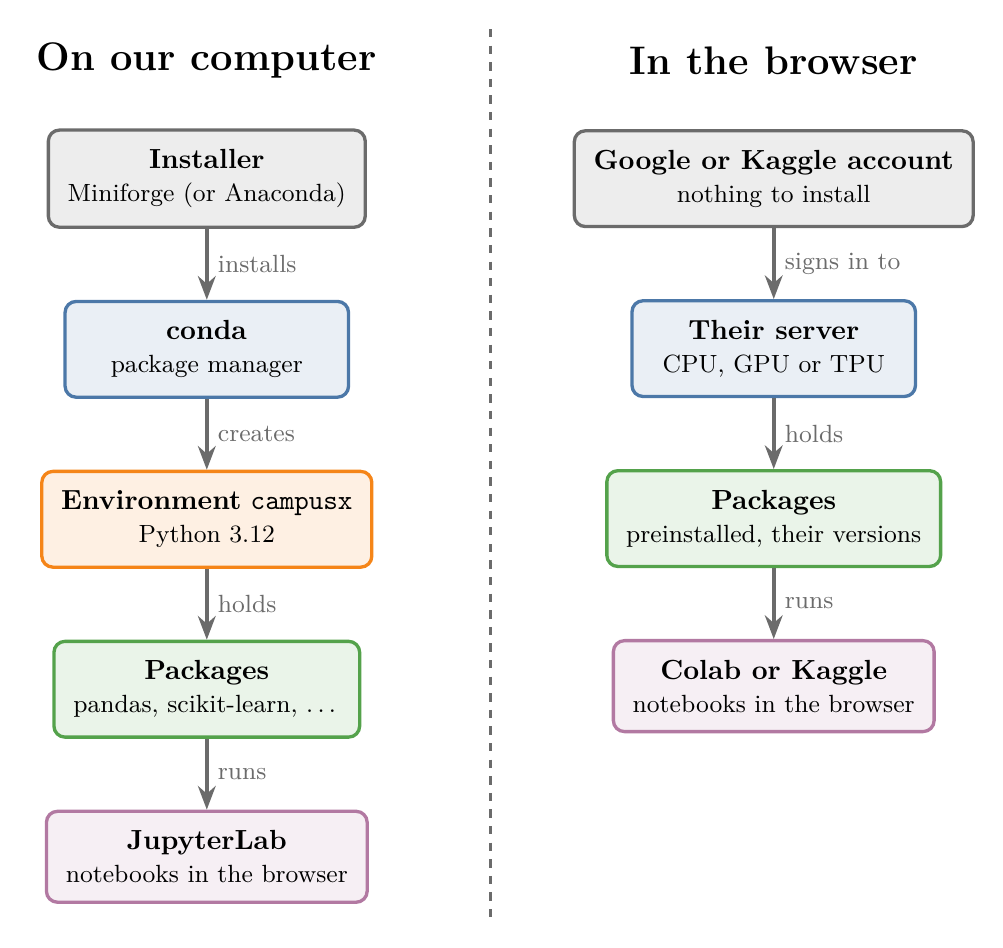
\begin{tikzpicture}[node distance=0.9cm]
  % local path
  \node[title] (lt) at (0,1.5) {On our computer};
  \node[box=cgrey, minimum width=3.6cm] (inst) at (0,0) {\textbf{Installer}\\{\small Miniforge (or Anaconda)}};
  \node[box=cblue, minimum width=3.6cm, below=of inst] (conda) {\textbf{conda}\\{\small package manager}};
  \node[box=corange, minimum width=3.6cm, below=of conda] (env) {\textbf{Environment} \texttt{campusx}\\{\small Python 3.12}};
  \node[box=cgreen, minimum width=3.6cm, below=of env] (pkg) {\textbf{Packages}\\{\small pandas, scikit-learn, \dots}};
  \node[box=cpurple, minimum width=3.6cm, below=of pkg] (jup) {\textbf{JupyterLab}\\{\small notebooks in the browser}};
  \draw[arrow] (inst) -- node[note, right] {installs} (conda);
  \draw[arrow] (conda) -- node[note, right] {creates} (env);
  \draw[arrow] (env) -- node[note, right] {holds} (pkg);
  \draw[arrow] (pkg) -- node[note, right] {runs} (jup);
  % online path
  \node[title] (ot) at (7.2,1.5) {In the browser};
  \node[box=cgrey, minimum width=3.6cm] (acc) at (7.2,0) {\textbf{Google or Kaggle account}\\{\small nothing to install}};
  \node[box=cblue, minimum width=3.6cm, below=of acc] (srv) {\textbf{Their server}\\{\small CPU, GPU or TPU}};
  \node[box=cgreen, minimum width=3.6cm, below=of srv] (pre) {\textbf{Packages}\\{\small preinstalled, their versions}};
  \node[box=cpurple, minimum width=3.6cm, below=of pre] (nb) {\textbf{Colab or Kaggle}\\{\small notebooks in the browser}};
  \draw[arrow] (acc) -- node[note, right] {signs in to} (srv);
  \draw[arrow] (srv) -- node[note, right] {holds} (pre);
  \draw[arrow] (pre) -- node[note, right] {runs} (nb);
  \draw[cgrey, dashed, line width=1pt] (3.6,1.9) -- (3.6,-9.4);
\end{tikzpicture}
\end{document}
